\chapter{Implementierung}
In diesem Kapitel wird die Implementierung der Methode näher erläutert. Bei der Implementierung werden alle Konzepte aus dem
Kapitel Konzeption angewendet.

% \section{Spiel-Datensatz}
% Für die Erstellung des Spiel-Datensatzes würde die Bibliothek ``Matplotlib''\footnote{https://matplotlib.org/} verwendet.

% \begin{lstlisting}[caption={Klasse Agent - Tensorflow Graph}, captionpos=b, label={lst:tf_graph_save}]
%   COLORS = [(236, 245, 66), (141, 245, 66), (245, 69, 66)]

%   for i in range(RANGE):
%     image = Image.new('RGB', (32, 32), 'black')
%     idx = np.random.randint(3)
%     x1 = np.random.randint(32)
%     y1 = np.random.randint(32)
%     x2 = np.random.randint(32)
%     y2 = np.random.randint(32)
  
%     draw = ImageDraw.Draw(image)
%     draw.rectangle((x1, y1, x2, y2), fill=COLORS[idx])
% \end{lstlisting}

\section{Binning}
Das Binning ist eine wichtige Komponente der Methode, dass mit Hilfe der ``numpy'' Bibliothek implementiert wurde. Als erstes wird 
anhand der Anzahl von Bins ($n\_bins$) die Breite ($B$) und Höhe ($H$) des \gls{grid}s, das auf der Abbildung \ref{image:bins} zu sehen ist,
mit Hilfe der Wurzel berechnet. Es wird angenommen dass $B = H$.
Nachdem die Breite des \gls{grid}s berechnet wurde, wird der Intervall von $[0, 1]$ in $B$ gleich große Intervalle aufgeteilt. Als nächstes
wird mit Hilfe der \textit{digitize} Funktion, der Intervall Index der jeweiligen $a, b$ Farbkanal Wert von jedem Pixel kalkuliert. 
Abschließend werden beide Indices zu einem Bin Index auf dem \gls{grid} umgewandelt. Der Output ist ein kodiertes Bild mit einem Bin Index per Pixel.
\\

\begin{listing}[H]
  \begin{minted}{python}
    # a, b sind die Koordinaten der Farbkanäle auf dem Grid
    def calculate_bin(a, b, width):
      return (width * b) + a
  
    def encode_bins(ab_image, n_bins):
      B = np.sqrt(n_bins).astype(int)
  
      # Intervall in gleich große Intervalle aufteilen
      interval = np.linspace(0, 1, B+1)
  
      # Indices für jeweils a, b Kanäle berechnen
      indices = np.digitize(ab_image, interval) - 1
  
      # Bin Index berechnen
      bins = np.vectorize(calculate_bin)(indices[:,:,0], indices[:,:,1], B)
  
      return bins
  \end{minted}
  \captionof{lstlisting}{Binning eines normalisierten Lab Bildes}
\end{listing}

\subsection{Umwandlung von Bin zu Farbe}
Für die Umwandlung werden vor dem Training alle Farben von den Trainingsbilder in Bins klassifiziert. Es wird ein Python Dictionary mit Bin
Indices als Key und einem 2-Dimensionalen Array mit einem Array pro Farbkanal als Value erzeugt.

\begin{listing}[H]
  \begin{minted}{python}
    bin_colors = {i: [[], []] for i in range(n_bins)}
  \end{minted}
  \captionof{lstlisting}{Leeres Dictionary Erzeugung für \textit{n_bins}}
\end{listing}

Anschließend werden die Farben von jedem Farbkanal in den jeweiligen Bin Array zugeordnet. Als letztes wird den Durchschnitt pro Bin Index
und Farbkanal berechnet. Der Dictionary beinhaltet abschließend ein Array mit 2 einzelne Werte für den jeweiligen Farbkanal pro Bin Index.
Somit kann unkompliziert ein Bin in eine Farbe umgewandelt werden.

\begin{listing}[H]
  \begin{minted}{python}
    a_color = bin_colors[bin_index][0]
    b_color = bin_colors[bin_index][1]
  \end{minted}
  \captionof{lstlisting}{Bin zu Farbe Umwandlung}
\end{listing}

Der gleiche Vorgang wird für den Modus angewendet. Um verschiedene Farben erzeugen zu können werden den Durchschnitt und der Modus mit einem
Temperatur Wert interpoliert.

\begin{listing}[H]
  \begin{minted}{python}
    a_distance = a_mode - a_mean
    b_distance = b_mode - b_mean

    a = a_mode - (a_distance * T)
    b = b_mode - (b_distance * T)
  \end{minted}
  \captionof{lstlisting}{Bin zu Farbe Berechnung mit einem Temperaturwert}
\end{listing}

\section{Datensätze}
Die Datensätze werden mit Hilfe der ``torchvision'' Bibliothek von PyTorch importiert und transformiert. Für das Importieren wurde eine
``ImageFolder'' implementiert, der die Bilder importiert, transformiert, normalisiert und in Bins kodiert. Der Output von den ``ImageFolder''
sind das Graustufenbild, das Bild mit den ``ab'' Farbkanäle und das in Bins kodierte Bild.

Mit Hilfe eines ``DataLoaders'' werden die Datensätze in Batches aufgeteilt und gemischt.

\section{Netzwerkarchitektur}
Für dieser Arbeit wurden 2 U-Nets mit verschiedene Größen verwendet. Ein U-Net für $ 32 \times 32 $ Bilder und ein U-Net für $ 128 \times 128 $ 
Bilder. Außerdem wurde das U-Net für $ 32 \times 32 $ Bilder angepasst damit es mit ein MSE Loss verwendet werden kann. Bei der Anpassung wurde
der Output Volumen zu $ W_{Input} \times H_{Input} \times 2 $ geändert, wobei das Netzwerk direkt die Werte für die ``ab'' Farbkanäle vorhersagt.
Bei der Verwendung von einem MSE Loss wird Binning nicht verwendet.
 
\subsection{ConvBlock}
Das Kernstück eines U-Nets ist der sogenannte ConvBlock. Ein ConvBlock beinhaltet zwei hintereinander geschaltete Blöcke, die wiederrum
aus einer Convolutional Layer mit $3 \times 3$ Filtern und Stride 1, gefolgt von ReLU und Batch Normalisation bestehen. 
Die Convolutional Layers verwenden Padding um die Dimensionen von dem Input nicht zu verändern. Die Layers wurden mit den PyTorch 
Klassen \textit{Conv2d}, \textit{BatchNorm2d} und die Funktion \textit{relu} implementiert. Das ConvBlock wird mit einer Klasse implementiert
die wiederrum von der Oberklasse \textit{torch.nn.Module} erbt.

\begin{figure}[H]
  \centering
  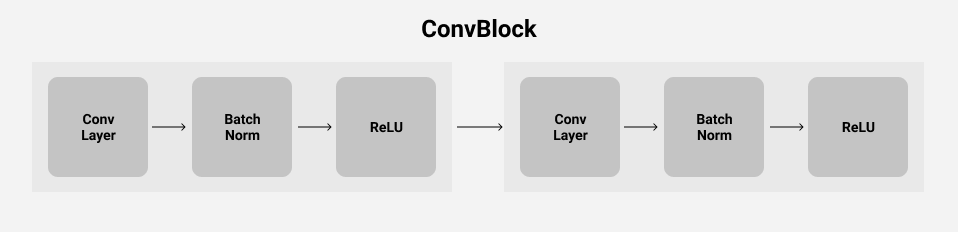
\includegraphics[width=1\textwidth]{resources/networks/convblock.png}
  \caption{ConvBlock}
  \label{image:convBlock}
\end{figure}

\subsection{U-Net}
Das U-Net wird mit den Spezifikationen aus \ref{section:u-net} implementiert. Dies geschieht mit einer Klasse, die von der Oberklasse
\textit{torch.nn.Module} erbt. Das U-Net verwendet neben den ConvBlocks, Max Pooling Layers mit einem $2 \times 2$ Filter und Stride 2,
um die Dimensionen in den Encoder zu halbieren. Die kleinste Größe der Feature Maps bei dem Encoder ist $8 \times 8$. 
Der Decoder verwendet ebenfalls neben den ConvBlocks, Transposed Convolutions mit $3 \times 3$ 
Filtern, Stride 2 und Padding 1, die die Größe der Feature Maps verdoppeln. Der letzte Layer ist ein Convolutional Layer mit $1 \times 1$ Filter, 
Stride 1 und Padding 0, der die
Wahrscheinlichkeitsverteilung pro Pixel generiert. Alle Transposed Convolutions werden mit den Outputs der ConvBlocks mit den gleichen
Dimensionen aus dem Encoder konkateniert. 
Es werden zwei verschieden große U-Nets implementiert, eins für $32 \times 32$ Bilder und eins für 
$128 \times 128$ Bilder.
\\
Die Max Pooling Layers wurden mit der \textit{MaxPool2d} Klasse und die Transposed Convolutions mit der \textit{ConvTranspose2d} implementiert.

\begin{figure}[H]
  \centering
  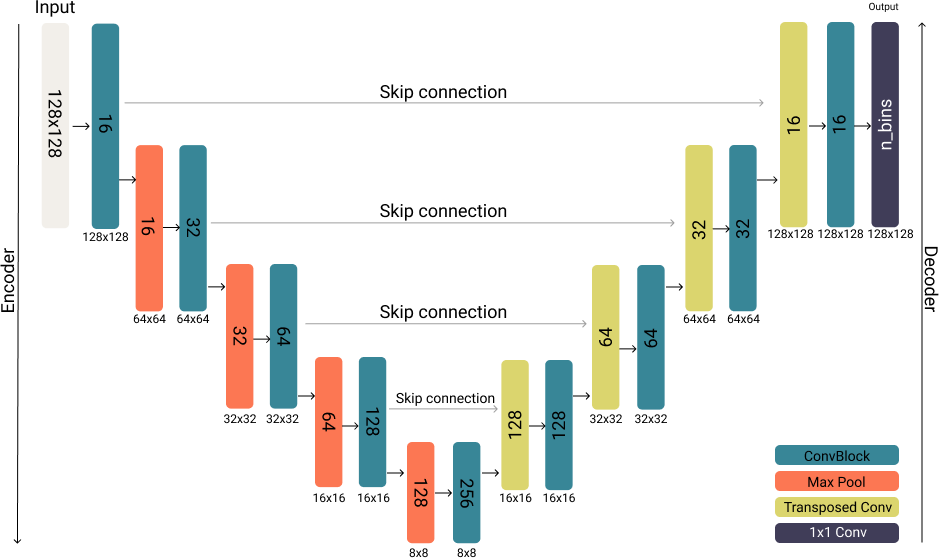
\includegraphics[width=1\textwidth]{resources/networks/128u-net.png}
  \caption{U-Net Architektur für $128 \times 128$ Input Bilder}
  \label{image:128u-net}
\end{figure}


% \section{Beispiel Unterkapitel}
% TODO